\section{Resultados}
\subsection{Contraste del simulador}
Las diez pruebas deterministas finalizaron correctamente. El contraste M/M/1 produjo los valores de la Tabla~\ref{tab:validacion}; los tres intervalos contienen sus referencias teóricas. Los errores relativos fueron inferiores al 0,4\,\%, lo que respalda el funcionamiento de la atención y las mediciones en el caso simplificado.

\begin{table}[t]
\centering\footnotesize
\caption{Contraste analítico M/M/1: 30 réplicas}
\label{tab:validacion}
\begin{tabular}{@{}lrrrr@{}}\toprule
Métrica & Teoría & Simulación & IC 95\,\% & Error (\%)\\\midrule
\inputrows{resultados/tabla_validacion.tex}
\bottomrule\end{tabular}
\end{table}

\subsection{Demanda, colas y distribución de trabajo}
La Tabla~\ref{tab:rendimiento} muestra los escenarios sin fallo. Las diferencias entre tamaños deben interpretarse junto con la carga: una configuración puede ser suficiente durante demanda baja y resultar inadecuada durante el pico. El aumento de capacidad no altera los tiempos de servicio generados; modifica la contención y la espera.

Con cuatro VMs y carga alta, MP redujo el p95 medio en \AltaRed{}\,\% respecto a RR. La diferencia pareada MP--RR fue \AltaDif{} s, con IC 95\,\% [\AltaLo{}, \AltaHi{}]. Durante el pico, cuatro VMs no aportaron capacidad suficiente y ambas políticas incumplieron el objetivo, pese a que la utilización media de toda la ventana no alcanzó el 100\,\%.

\begin{table}[t]
\centering\footnotesize
\caption{Rendimiento sin fallo: medias de 30 réplicas}
\label{tab:rendimiento}
\begin{tabular}{@{}lrlrrrr@{}}\toprule
Carga & VMs & Pol. & p95 (s) & $\overline Q$ & CPU (\%) & $G$ (\%)\\\midrule
\inputrows{resultados/tabla_rendimiento.tex}
\bottomrule\end{tabular}
\end{table}

La Fig.~\ref{fig:latencia} compara el p95 del perfil con pico, con y sin fallo. MP utiliza la ocupación observada para evitar destinos con mayor acumulación de trabajo; RR conserva la secuencia de turnos. Ambas políticas están limitadas por la capacidad total, de modo que una distribución diferente no elimina un déficit sostenido de procesamiento.

\begin{figure}[t]
\centering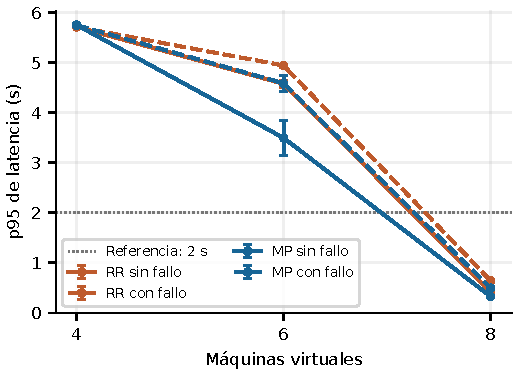
\includegraphics[width=\columnwidth]{figuras/latencia.pdf}
\caption{Latencia en el perfil con pico. Barras: IC puntual del 95\,\% para la media de p95 entre réplicas. La línea de 2 s es una referencia visual; la restricción formal se evalúa con $G$.}
\label{fig:latencia}
\end{figure}

\subsection{Fallo del host y evolución temporal}
La Fig.~\ref{fig:evolucion} presenta una réplica con entradas comunes y distintas configuraciones. El intervalo sombreado identifica el fallo del host 1. La pérdida de capacidad se superpone a la fase de demanda máxima; las colas muestran la capacidad del sistema para absorber y eliminar la acumulación. La ocupación de CPU se interpreta con relación a la capacidad disponible y a la contratada.

\begin{figure*}[t]
\centering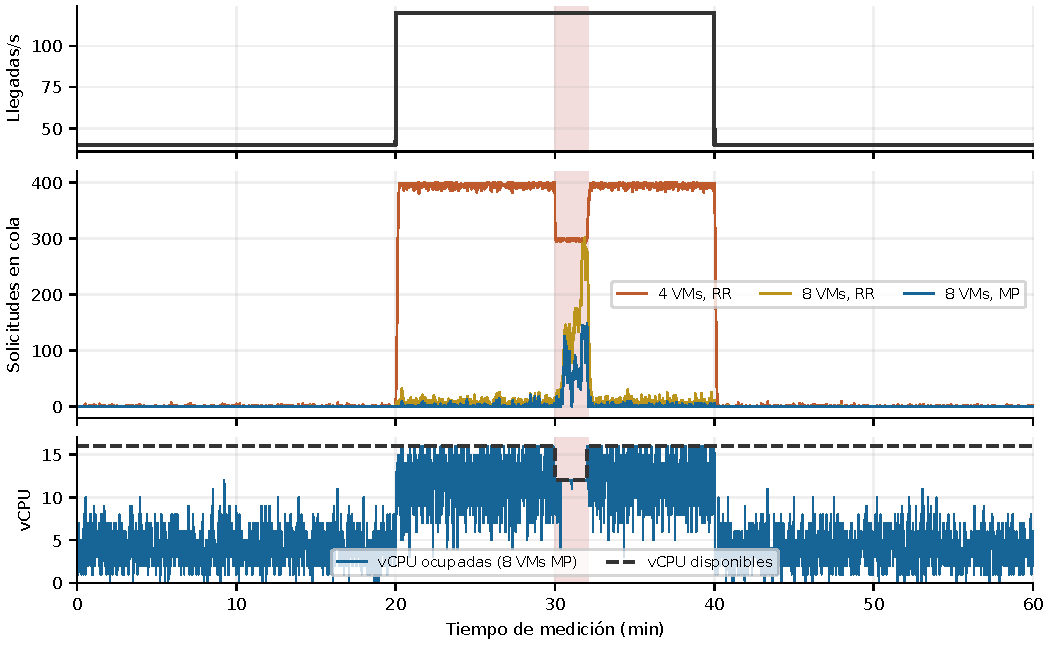
\includegraphics[width=.91\textwidth]{figuras/evolucion.pdf}
\caption{Evolución de una réplica del perfil con pico y fallo, semilla 0. La demanda aumenta en el minuto 20 y disminuye en el 40; el host 1 está caído entre los minutos 30 y 32. Las series se muestrean cada segundo para exposición y no sustituyen el análisis de las 30 réplicas.}
\label{fig:evolucion}
\end{figure*}

\subsection{Selección de la alternativa de menor costo}
La Tabla~\ref{tab:seleccion} resume, para cada alternativa, el mínimo éxito, el mínimo cumplimiento de rapidez y el máximo p95 medio entre los seis escenarios. Los extremos de una fila pueden corresponder a escenarios diferentes. Una alternativa es factible únicamente cuando todas sus medias de escenario satisfacen las restricciones.

\begin{table*}[t]
\centering\small
\caption{Evaluación exhaustiva de alternativas; costo sintético por horizonte común}
\label{tab:seleccion}
\begin{tabular}{@{}rcrrrrc@{}}\toprule
VMs & Política & Costo (u. m.) & Mín. $A$ (\%) & Mín. $G$ (\%) & Máx. p95 (s) & Factible\\\midrule
\inputrows{resultados/tabla_seleccion.tex}
\bottomrule\end{tabular}
\end{table*}

La regla de decisión seleccionó \ElegidaVM{} VMs y \ElegidaPolitica{}, con costo de \ElegidaCosto{} u. m. por ejecución. Su menor éxito fue \ElegidaA{}\,\%, su menor cumplimiento de dos segundos fue \ElegidaG{}\,\% y su máximo p95 medio fue \ElegidaP{} s. El costo depende del número de VMs, no de la política, por lo que el desempate mediante latencia distingue alternativas con igual aprovisionamiento.

Ambas políticas con ocho VMs resultaron factibles. En el pico con fallo, MP redujo el p95 medio en \PicoRed{}\,\% frente a RR; la diferencia pareada fue \PicoDif{} s, con IC 95\,\% [\PicoLo{}, \PicoHi{}]. Para la alternativa seleccionada, los mínimos límites inferiores puntuales fueron \ElegidaLCBA{}\,\% en éxito y \ElegidaLCBG{}\,\% en rapidez, por encima de sus respectivos umbrales.

\begin{figure}[t]
\centering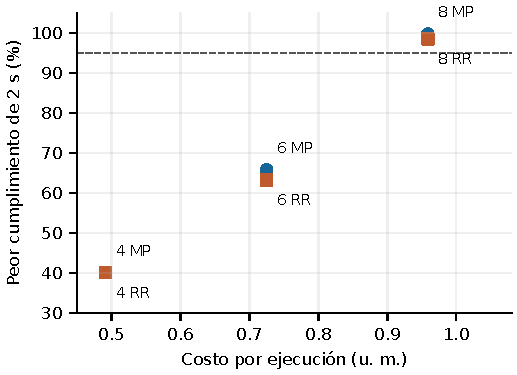
\includegraphics[width=\columnwidth]{figuras/costo_servicio.pdf}
\caption{Compromiso costo--rapidez. Cada punto es una configuración; el eje vertical recoge el peor $G$ medio entre escenarios. La línea discontinua marca el objetivo del 95\,\%; también se exige $A\geq99\,\%$.}
\label{fig:costo}
\end{figure}

Los CSV conservan las métricas por réplica. Los resúmenes, las diferencias pareadas y la selección se generan por programa; LaTeX importa directamente las tablas calculadas.

\subsection{Costo incremental de la capacidad}
Con el horizonte común de $T=1,16944$ h, cada VM adicional agrega \CostoVMAdicional{} u. m. por ejecución y el balanceador aporta \CostoBalanceador{} u. m. fijas. Los porcentajes siguientes se calcularon con los costos originales, antes de redondearlos para su presentación.

Pasar de seis a ocho VMs incrementó el costo de \CostoSeis{} a \CostoOcho{} u. m., un \AumentoSeisOcho{}\,\%. En la política MP, el peor cumplimiento de dos segundos aumentó de \GSeisMP{}\,\% a \ElegidaG{}\,\%. Dentro de los tamaños evaluados, ocho VMs fue la menor capacidad que satisfizo simultáneamente las restricciones~\eqref{eq:disp} y~\eqref{eq:rapidez} en todos los escenarios.

Reducir de ocho a cuatro VMs ahorra \AhorroOchoCuatro{}\,\%, pero con MP el peor cumplimiento cae a \GCuatroMP{}\,\% e incumple las restricciones. La selección considera costo de aprovisionamiento y factibilidad; no estima rentabilidad total, pues no incluye penalizaciones monetarias por errores o demora.
